\documentclass{beamer}
\usefonttheme[onlymath]{serif}
\usepackage[english]{babel}							%For internationalization
\usepackage[utf8]{inputenc}							%For character encoding
\usepackage{amsmath}								%For mathematical typesetting
\usepackage{amssymb}								%For mathematical typesetting
\usepackage{graphicx}								%For handling graphics
\usepackage{listings}

\newcommand{\be}{\begin{equation}}
\newcommand{\ben}[1]{\begin{equation}\label{#1}}
\newcommand{\ee}{\end{equation}}

\setbeamerfont{footnote}{size=\tiny}
\beamertemplatenavigationsymbolsempty
\setbeamerfont{page number in head/foot}{size=\large}
\setbeamertemplate{footline}[frame number]
\lstset{breaklines=true,basicstyle=\tiny}

\title
{A High-Order Fast Algorithm Approach for Computing Layer and Volume Potentials }
\author[Bevan] % (optional, for multiple authors)
{J.~Bevan, UIUC}
\institute[UIUC] % (optional)

\date[April, 2017] % (optional)
{\textit{CS 591 Seminar\\ April, 2017}}
\subject{Discontinuous Galerkin}

\begin{document}
\frame[plain,noframenumbering]{\titlepage}

\section{Introduction}

\subsection{Motivation} 
\frame{\frametitle{\subsecname}
\begin{itemize}
\item Evaluation of potentials (derived velocity field, electric potential, etc.) is an important physical consideration
\item Practical computational im[implementation faces two challenges: $\mathcal{O}(n^2)$ cost and integrable singularities
\end{itemize}

\begin{figure}
\centering
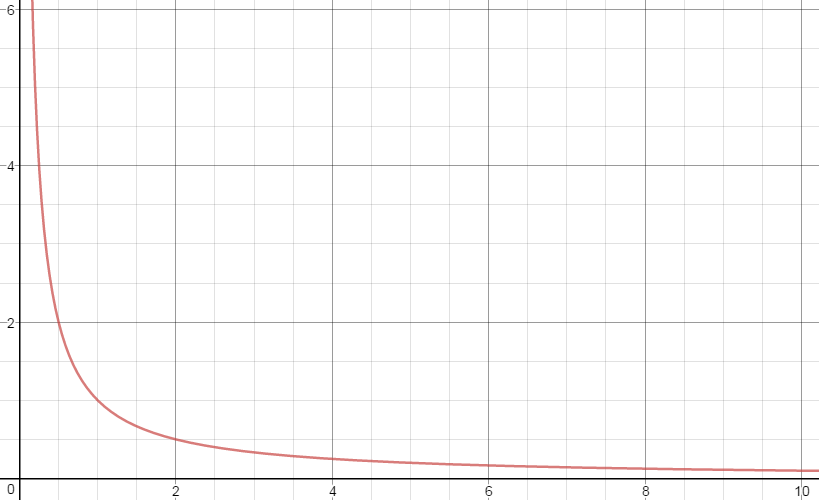
\includegraphics[width=1.5in]{Capture2.PNG}
\end{figure}

\begin{figure}
\centering
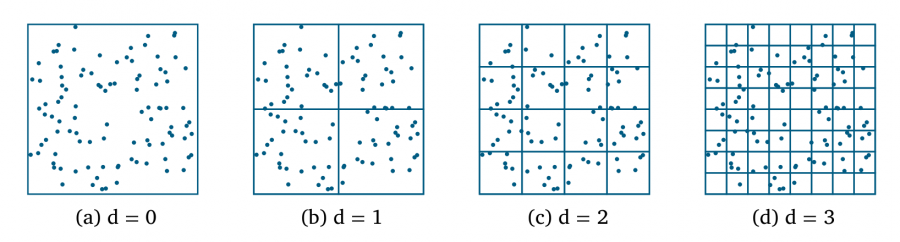
\includegraphics[width=4in]{FMM.PNG}
\end{figure}

\footnotetext{https://summerofhpc.prace-ri.eu/}
}

\subsection{QBX} 
\frame{\frametitle{\subsecname}

\begin{figure}
\centering
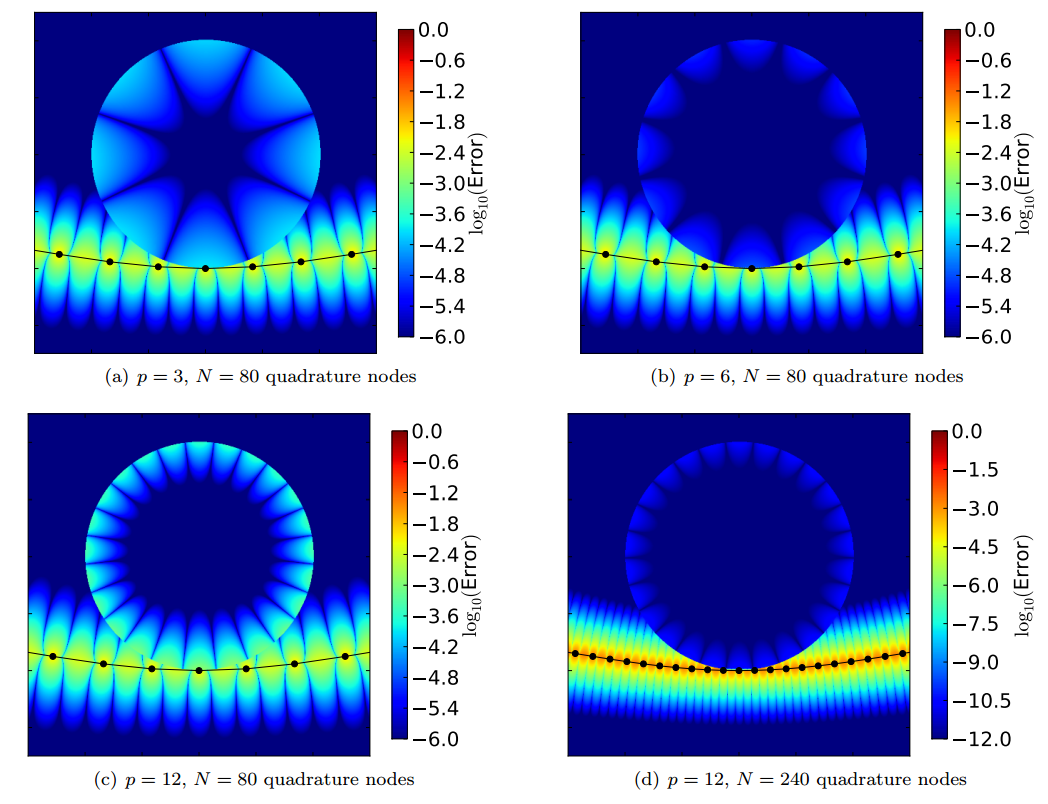
\includegraphics[width=4in]{Capture.PNG}
\end{figure}

\footnotetext{Klöckner, Andreas, et al. "Quadrature by expansion: A new method for the evaluation of layer potentials." Journal of Computational Physics 252 (2013): 332-349.}
}

\subsection{QBX Considerations} 
\frame{\frametitle{\subsecname}
\begin{itemize}
\item Global vs local approaches involve all source points, or only the "near-field" respectively
\item Layer potentials provide physical meaningful off-surface potential
\item Volume potentials involve arbitrary choice of "off-volume" potential
\end{itemize}
}

\subsection{Mesh Interaction} 
\frame{\frametitle{\subsecname}
\begin{itemize}
\item Given some mesh with a spatially varying blob of "charge", local QBX needs only some of the mesh
\item How are varying intersection cases to be handled?
\item How conservative/efficient can one be with intersections?
\end{itemize}
}

\subsection{Mesh Interaction} 
\frame{\frametitle{\subsecname}

\begin{figure}
\centering
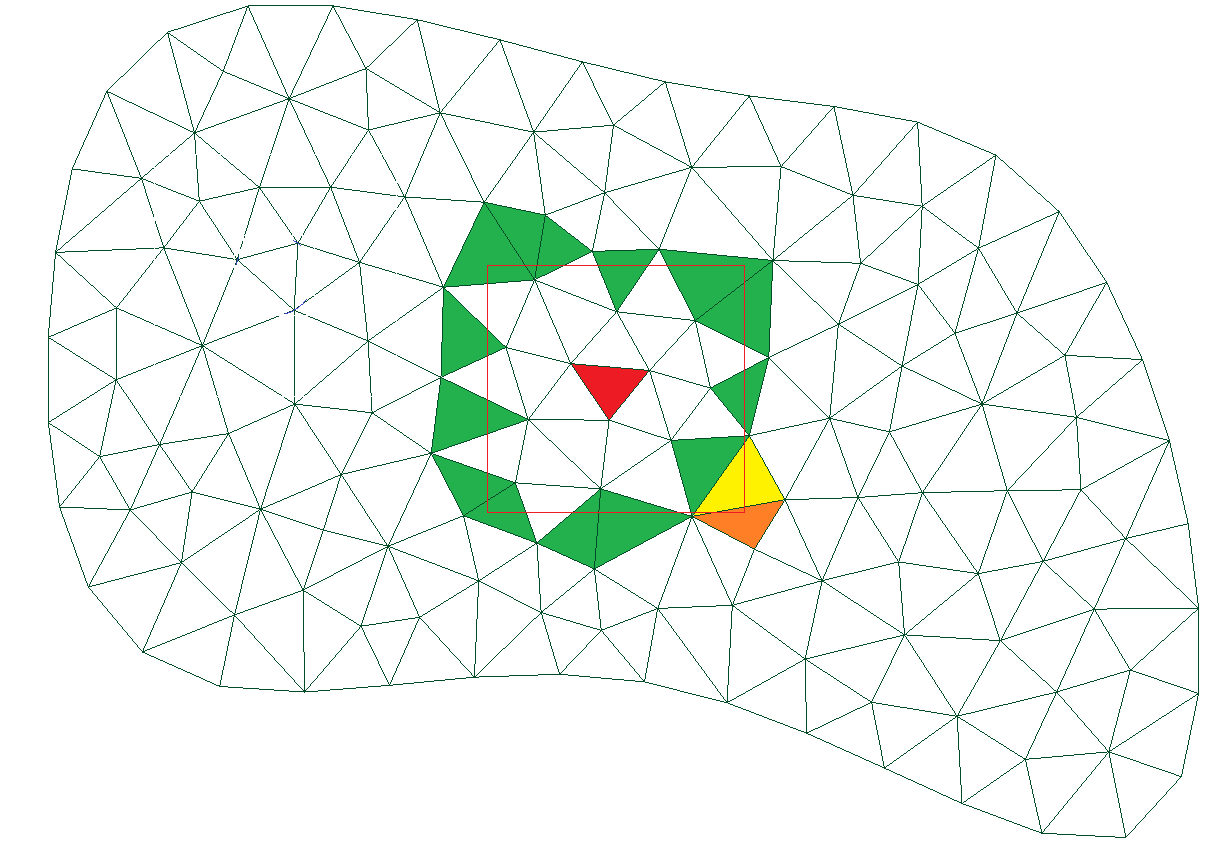
\includegraphics[width=4in]{area1.PNG}
\end{figure}
}

\subsection{FMM-QBX Interaction} 
\frame{\frametitle{\subsecname}

\begin{figure}
\centering
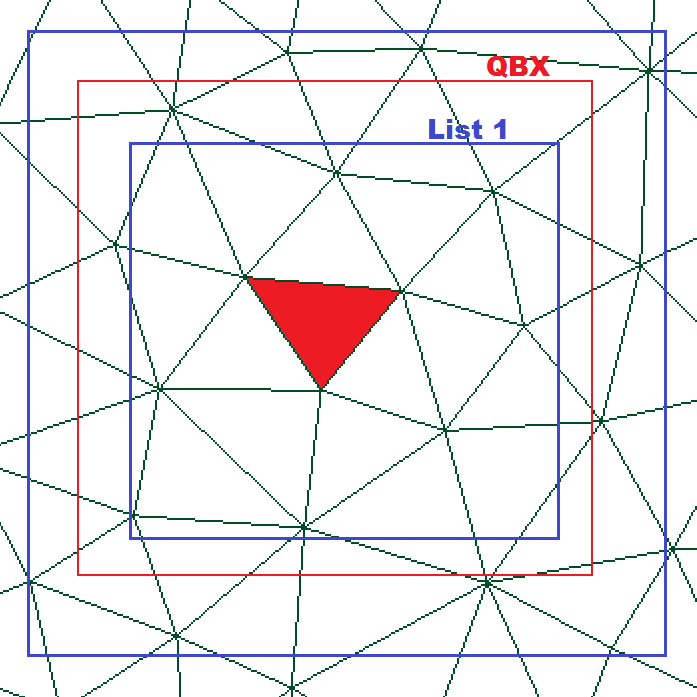
\includegraphics[width=3in]{corner.PNG}
\end{figure}
}

\subsection{Corrected FMM Contributions} 
\frame{\frametitle{\subsecname}

\begin{figure}
\centering
\includegraphics[width=4in]{Figure_1.PNG}
\end{figure}
}

\subsection{QBX Contributions} 
\frame{\frametitle{\subsecname}

\begin{figure}
\centering
\includegraphics[width=4in]{Figure_2.PNG}
\end{figure}
}

\subsection{QBX-FMM Overlap Corrections} 
\frame{\frametitle{\subsecname}

\begin{figure}
\centering
\includegraphics[width=4in]{Figure_3.PNG}
\end{figure}
}

\subsection{Result of Combinations} 
\frame{\frametitle{\subsecname}

\begin{figure}
\centering
\includegraphics[width=4in]{Figure_C.PNG}
\end{figure}
}



\end{document}